\documentclass[a4paper,oneside]{book}
\usepackage{anysize}
\usepackage{lastpage}
\usepackage{fancyhdr}
\usepackage{polyglossia}
\setdefaultlanguage[variant=uk]{english}
\usepackage{fontspec}
\usepackage{color}
\definecolor{bkg}{rgb}{0.9,0.9,0.9}
\definecolor{cmt}{rgb}{0.0,0.6,0.0}
\definecolor{boxbkg}{rgb}{0.9,0.95,1.0}
\usepackage{fancybox}
\usepackage{mdframed}
\usepackage{listings}
\defaultfontfeatures{Ligatures=TeX}
\usepackage{graphicx}
\graphicspath{{./logo/}{./img/}}
\usepackage[x11names]{xcolor}
\usepackage[colorlinks=true]{hyperref}
\usepackage{framed}
\usepackage{float}
\usepackage{wrapfig}
\restylefloat{figure}
\usepackage{makeidx}
\usepackage{listings}
\usepackage{amsmath}

\setlength{\emergencystretch}{3em}

\newtoggle{InString}{}% Keep track of if we are within a string
\togglefalse{InString}% Assume not initally in string

\lstset{
    backgroundcolor=\color{bkg},
    basicstyle=\small\ttfamily,
    breaklines=true,
    columns=fullflexible,
    numbers=left,
    numberstyle=\tiny,
    keywordstyle=\color{blue},
    commentstyle=\color{cmt},
    stepnumber=5,
    captionpos=b,
}
\lstdefinelanguage{json}{
    string=[s]{"}{"},
    showstringspaces=false,
    stringstyle=\color{purple},
    morecomment=[s][\color{black}\ttfamily]{\ \ \"}{\"},
    morecomment=[s][\color{purple}\ttfamily]{\ \ \ \ \ \"}{\"},
    keywords=[1]{true, false},
    keywordstyle=[1]\color{cyan},
    columns=flexible,
    keepspaces=true,
    morecomment=[l]{//},
}
\usepackage{caption}
\usepackage{subcaption}

\marginsize{1.5cm}{1.5cm}{0.5cm}{1.7cm}
\pagestyle{plain}
\setmainfont{Reporter}
\makeindex

\begin{document}
\begin{figure}[h]
  \includegraphics[width=\textwidth]{doc_head.jpg}
\end{figure}

\parindent=0pt
\parskip=0.25cm

\begin{center}
\fontsize{20}{21}\selectfont

\textbf{Gaze Recording with Tobii Eye Trackers}:\\
Usage of \textbf{screen based Tobii Eye Trackers}\\
from within a 3rd party program\\
\vskip 6mm
Tutorial
\vskip 6mm

\fontsize{13}{14}\selectfont
Simon Maurer - \texttt{simon.maurer@humdek.unibe.ch}\\
\today
\end{center}

\tableofcontents

%==============================================================================
\chapter{Introduction}\label{sec.intro}
This documents describes how to use the \href{https://www.tobii.com/products/eye-trackers/screen-based/tobii-pro-spark}{Tobii Eye Tracker Spark} and the \href{https://tobiigaming.com/eye-tracker-4c/}{Tobii Eye Tracker 4C} to record gaze data of a subject and (optionally) feed the gaze data to the mouse device.
This allows to use the eye tracker to control the mouse pointer position such that the mouse pointer is placed at the screen coordinates where the subject is gazing at.
This documentation comes with a set of tools (executable .exe files) that provide this functionality as well as some auxiliary tools that help to calibrate and test the eye tracker.

The project aims at providing a set of executables which allow to use the Eye Trackers in conjunction with third party applications that allow to execute external programs.
Specifically, \href{http://www.ztree.uzh.ch/en.html}{ztree} or \href{https://osdoc.cogsci.nl/3.3/}{openseame}.
The following set of executables are provided:
\begin{description}
    \item[TobiiCalibrate.exe] This program is a simple wrapper for the Tobii calibration tool.
        It launches the calibration GUI where the subject is led through the calibration process.
        The calibration data is stored in the current profile of the eye tracker engine.
        \textbf{Attention:} Make sure to to have the \href{https://www.tobii.com/products/software/applications-and-developer-kits/tobii-pro-eye-tracker-manager}{Tobii Pro Eye Tracker Manager} of version 2.6 or later installed.
    \item[Gaze.exe] This program uses the \href{http://developer.tobii.com/tobii-pro-sdk/}{Tobii Pro SDK} to extract the gaze position on the screen where the subject is looking at.
        The extracted data is recorded and stored to a file.
        Optionally, the mouse cursor position is updated to this position such that the mouse cursor is controlled by the gaze of the subject.
        Instead of using an eye tracker device it is also possible to simply log the mouse coordinates.

        \texttt{Gaze.exe} runs infinitely until it is terminated by an external command.
        This should \textbf{not} be done with a forced kill (e.g.~by executing the command \texttt{taskkill /F /IM Gaze.exe} or by killing the task with the task manager) because it prevents the program from terminating gracefully.
        This as several consequences:
        \begin{itemize}
            \item open files are not closed properly and the data stream is cut off. This can lead to corrupt files.
            \item if the feature of hiding the mouse pointer is used, the mouse will remain hidden.
            \item memory is not freed properly.
        \end{itemize}
        Instead the program \texttt{GazeControls.exe /command TERMINATE} should be used.

        The application takes the following two input arguments:
        \begin{description}
            \item[subject]
                A subject code which will be used to prefix the output files.
            \item[outputPath]
                The location where the output files will be stored.
                Note that this can also be configured through the configuration option \texttt{DataLogPath} (see Chapter \ref{sec.config}).
        \end{description}
    \item[GazeControl.exe] This program allows to interact with Gaze.exe.
        Run GazeControl.exe with the argument \texttt{/command <COMMAND>} to perform the command in Gaze.exe.
        Passing an argument to an application can be done in command line or by crating a shortcut to the program.
        Corresponding shortcuts for all available \texttt{<COMMAND>}s are provided in the release package.
        The following \texttt{<COMMAND>}s are available:
        \begin{description}
            \item{\texttt{CUSTOM\_CALIBRATE}} uses the \href{http://developer.tobii.com/tobii-pro-sdk/}{Tobii Pro SDK} and launches a custom calibration process which allows to calibrate the eye tracker without having to rely on the calibration software provided by Tobii.
            \item{\texttt{VALIDATE}} uses the \href{https://github.com/tobiipro/prosdk-addons-dotnet/}{Tobii Pro SDK Addon} and launches a validation process.
            \item{\texttt{DRIFT\_COMPENSATION}} launches a custom drift compensation process to compensate gaze drifts that may occur during experimentation.
            \item{\texttt{GAZE\_RECORDING\_DISABLE}} requests Gaze.exe to stop recording gaze data.
                Gaze.exe will continue to run (and update the mouse pointer if configured accordingly) but no longer store gaze data to the disk.
            \item{\texttt{GAZE\_RECORDING\_ENABLE}} requests Gaze.exe to start recording gaze data.
            \item{\texttt{MOUSE\_TRACKING\_DISABLE}} requests Gaze.exe to stop updating the mouse pointer by the gaze position.
            \item{\texttt{MOUSE\_TRACKING\_ENABLE}} requests Gaze.exe to start updating the mouse pointer by the gaze position.
            \item{\texttt{RESET\_DRIFT\_COMPENSATION}} resets the drift compensation computed with the command \texttt{DRIFT\_COMPENSATION}.
            \item{\texttt{TERMINATE}} requests Gaze.exe to close gracefully and logs these events to the log file.
            \item{\texttt{SET\_TAG\ <TAG>}} sets a custom tag \texttt{<TAG>} which will be added to each data sample in the output file (use argument \texttt{/value} to define the \texttt{<TAG>}).
            \item{\texttt{SET\_TRIAL\_ID <ID>}} sets a trial ID integer number \texttt{<ID>} which will be added to each data sample in the output file (use argument \texttt{/value} to define the \texttt{<ID>}).
            \item{\texttt{RESET\_START\_TIME} allows to reset the relative timestamp. The relative timestamp can also be reset by passing the argument \texttt{/reset} to the application with any of the above commands.
        \end{description}
    \item[ShowMouse.exe] This program allows to restore the standard mouse pointer.
        It might be useful if the program \texttt{Gaze.exe} crashes or is closed forcefully such that the mouse pointer is not restored after terminating.
        The subject might end up with a hidden mouse pointer.
        A good solution for such a case is to install a shortcut to \texttt{ShowMouse.exe} on the desktop in order to execute it with the keyboard.
\end{description}

%------------------------------------------------------------------------------
\section{Requesting a TPF GitLab Account}
\label{sec.gitlab}
The necessary code for what is described in this document is contained in a \texttt{GitLab} instance running on the \href{http://phhum-g111-nns.unibe.ch:10012/}{TPF server}\footnote{http://phhum-g111-nns.unibe.ch:10012/}.

Please send a mail to \href{tpf@humdek.unibe.ch}{TPF}\footnote{tpf@humdek.unibe.ch} with a request, specifying your name and the name of the TPF project you are interested in (e.g~\texttt{tobii\_eye\_tracker\_gaze}).

%==============================================================================
\chapter{Quick Start}
\label{sec.quick}
In order to get started with Tobii eye tracking the following installation steps need to be performed:
\begin{itemize}
    \item Install the \href{https://www.tobii.com/products/software/applications-and-developer-kits/tobii-pro-eye-tracker-manager}{Tobii Pro Eye Tracker Manager} application.
    \item Setup the \emph{Tobii Pro Spark} device with the following steps:
        \begin{itemize}
            \item Connect the \emph{Tobii Pro Spark} device to the computer.
                Make sure that the device is connected to a powered USB-type A port or, alternatively, use the provided USB-type A to USB-type C adapter and connect the device to a USB-type C port.
            \item Launch the Tobii Pro Eye Tracker Manager application
            \item Click on the button \emph{Install New Eye Tracker}
            \item Select the device \emph{Tobii Pro Spark}
            \item Click Install
            \item Now the eye tracker device should appear in the list.
                Click on the device and setup the screen calibration.
            \item Perform the device calibration and verify the gaze accuracy through the built-in gaze visualization
        \end{itemize}
    \item Setup the \emph{Tobii Eye Tracker 4C} device with the following steps:
        \begin{itemize}
            \item Install the \href{https://files.update.tech.tobii.com/Tobii.IS4C.Offline.Installer_4.124.0.15937.msi}{Tobii Experience} software.
                This software comes with the device driver for the \emph{Tobii Eye Tracker 4C}, however, it is only available as a beta version and is no longer maintained.
            \item Connect the \emph{Tobii Eye Tracker 4C} device to the computer.
            \item Now the eye tracker device should appear in the list of available devices in the \emph{Tobii Pro Eye TRacker Manager} application.
                Click on the device and setup the screen calibration.
            \item Perform the device calibration and verify the gaze accuracy through the built-in gaze visualization
        \end{itemize}
    \item Install the \href{http://phhum-g111-nns.unibe.ch:10012/TBI/TBI-tobii_eye_tracker_gaze}{Gaze toolset} provided by the TPF.
        To install the toolset \href{http://phhum-g111-nns.unibe.ch:10012/TBI/TBI-tobii_eye_tracker_gaze/tree/master/release}{download}\footnote{http://phhum-g111-nns.unibe.ch:10012/TBI/TBI-tobii\_eye\_tracker\_gaze/tree/master/release} the latest version (requires a subscription, see Section~\ref{sec.gitlab}) and extract all files to an installation path of your choosing.
        The Gaze toolset installation path will be referred to as \texttt{<Gaze toolset path>} throughout this document.
\end{itemize}


%------------------------------------------------------------------------------
\section{Quick Start with ztree}
\label{sec.quick.ztree}
In order to get started with a quick experiment you need the following things (\emph{server} refers to the machine running \texttt{ztree} and \emph{client} refers to the machines running \texttt{zleaf}):
\begin{itemize}
    \item a \href{http://www.ztree.uzh.ch/en.html}{ztree} installation with a server and one or more clients.
        To install \texttt{ztree} download the latest \texttt{ztree} version from the \href{https://www.uzh.ch/ztree/ssl-dir/index.php}{download secetion}\footnote{https://www.uzh.ch/ztree/ssl-dir/index.php} (requires a license and a login, see Section~\ref{sec.ztree}) and extract the server file \texttt{ztree.exe} to the chosen installation path on the server and the client file \texttt{zleaf.exe} to the chosen installation path on each client.
        Throughout this documentation the installation paths of the \texttt{ztree} client and server will be referred to as \texttt{<zleaf path>} and \texttt{<ztree path>}, respectively.
    \item the ztree sample file.
        The file is located in \texttt{<Gaze toolset path>\textbackslash sample\textbackslash template.ztt}.
        Make sure to change the \texttt{Path} variable in \texttt{Background} of the sample file such that it points to \texttt{<Gaze toolset path>}.
\end{itemize}

The provided sample \texttt{ztree} program performs the following stages:
\begin{description}
    \item[Initialise Eye Tracker]
        Starts the Gaze.exe application to run in the background during the experiment.
        Note that a sleep of five seconds is introduced here to give the eye tracker time to initialize.
    \item[Calibrate Eye Tracker]
        Runs the command \texttt{GazeControl.exe /command CUSTOM\_CALIBRATE} to start the custom calibration.
    \item[Enable Mouse Tracking]
        Runs the command \texttt{GazeControl.exe /command MOUSE\_TRACKING\_ENABLE}.
        The gaze of the subject is tracked and transformed to mouse coordinates which allows to control the mouse pointer with the gaze of the subject.
    \item[Terminate]
        Runs the command \texttt{GazeControl.exe /command TERMINATE} to gracefully shutdown the gaze application and conclude this simple \texttt{ztree} program.
\end{description}

The behaviour of the Gaze toolset can be configured with a configuration file (see Chapter~\ref{sec.config} for more details).
A sample configuration file is provided in \texttt{<Gaze toolset path>\textbackslash sample\textbackslash config.json} that can be modified to suit different requirements.
Copy the configuration file either to \texttt{<Gaze toolset path>} or \texttt{<zleaf path>} and modify it there.

%------------------------------------------------------------------------------
\subsection{Requesting Access to the Latest \texttt{ztree} Release}
\label{sec.ztree}
To download the latest release of the \texttt{ztree} software a login must be requested \href{https://www.uzh.ch/ztree/ssl-dir/index.php?action=obtain}{here}\footnote{https://www.uzh.ch/ztree/ssl-dir/index.php?action=obtain}.
Make a careful note of the terms and conditions.

%------------------------------------------------------------------------------
\section{Quick Start with opensesame}
\label{sec.quick.opensesame}
In order to get started with a quick experiment the following steps are required:
\begin{itemize}
    \item Install the latest version of \href{https://osdoc.cogsci.nl/3.3/download/}{opensesame} with your preferred installation method.
    \item As a starting point use the provided opensesame sample file.
        The file is located in\\ \texttt{<Gaze toolset path>\textbackslash sample\textbackslash template.osexp}.
        Make sure to change the \texttt{gazeAppPath} variable in \texttt{gaze\_initialisation} of the sample file such that it points to \texttt{<Gaze toolset path>}.
\end{itemize}

The provided sample \texttt{opensesame} program includes the following python scripts:
\begin{description}
    \item[gaze\_start]
        Sets the \texttt{gazeAppPath} variable during prepare stage and then starts the gaze application.
        The application will run in the background during the experiment.
        Note that the \texttt{subject\_nr} variable and the \texttt{experiment\_path} variable are passed as arguments to the application.
        The former is used to prefix the output file names with the subject number and the latter is used as location to store the output files.
        Also, note that the log files are stored at the \texttt{gazeAppPath}.
        Further, note that a sleep of three seconds is introduced here to give the eye tracker time to initialize.
    \item[gaze\_calibration]
        Runs the command \texttt{GazeControl.exe /command CUSTOM\_CALIBRATE} to start the custom calibration.
    \item[gaze\_validation]
        Runs the command \texttt{GazeControl.exe /command VALIDATE} to start the validation.
    \item[loop]
        Loops over a table of trial IDs
        \begin{description}
            \item[gaze\_drift\_compensation]
                Runs the command \texttt{GazeControl.exe /command DRIFT\_COMPENSATION} to start the drift compensation process.
            \item[set\_trial\_id]
                Runs the command \texttt{GazeControl.exe /command SET\_TRIAL\_ID /value <ID>} to communicate a trial ID to the gaze application.
                Note that \texttt{<ID>} is an ID extracted from the loop table.
            \item[gaze\_recording\_enable]
                Runs the command \texttt{GazeControl.exe /command GAZE\_RECORDING\_ENABLE} to start storing gaze data to the disk.
            \item[loop]
                Loops over a table of labels
                \begin{description}
                    \item[set\_label]
                        Runs the command \texttt{GazeControl.exe /command SET\_LABEL /value <LABEL>} to communicate a label to the gaze application.
                        Note that \texttt{<LABEL>} is a label extracted from the loop table.
                    \item[timeout]
                        Waits for one second.
                \end{description}
            \item[gaze\_recording\_disable]
                Runs the command \texttt{GazeControl.exe /command GAZE\_RECORDING\_DISABLE} to stop storing gaze data to the disk.
        \end{description}
    \item[gaze\_stop]
        Runs the command \texttt{GazeControl.exe /command TERMINATE} to gracefully shutdown the gaze application.
\end{description}

The behaviour of the Gaze toolset can be configured with a configuration file (see Chapter~\ref{sec.config} for more details).
A sample configuration file is provided in \texttt{<Gaze toolset path>\textbackslash sample\textbackslash config.json} that can be modified to suit different requirements.
Copy the configuration file either to \texttt{<Gaze toolset path>} or \texttt{<zleaf path>} and modify it there.


%==============================================================================
\chapter{Use Gaze Toolset in 3rd Applications}
\label{sec.gazetomouse}
This chapter provides instructions of how to use the Gaze toolest in a 3rd party application.
The gaze toolest contains several executable applications which can be started from within 3rd party applications to add eye tracker support.
The two main pieces is the \texttt{CustomCalibration} application which allows to calibrate the eye tracker and the \texttt{Gaze} application which allows to record gaze data.
The applications \texttt{GazeClose}, \texttt{GazeRecordingDisable}, \texttt{GazeRecordingEnable}, \texttt{MouseTrackingDisable}, and \texttt{MouseTrackingEnable} only work in conjunction with the \texttt{Gaze} application and are used to control the \texttt{Gaze} application (refer to Section \ref{sec.intro} for an overview).

%------------------------------------------------------------------------------
\section{Basic Principles of a Screen Based Tobii Eye Tracker}
\label{sec.eyetracker}
The eye tracker is mounted on the bottom of the screen such that its cameras are able to capture the eyes of the subject.
Several infrared LEDs are visible once the device is connected and properly working (see Figure~\ref{fig.eyetracker}).
This requires the Tobii software to be installed and running.
\begin{figure}[ht]
    \centering
    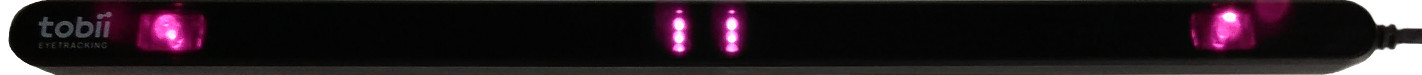
\includegraphics[width=0.95\textwidth]{eye_tracker.jpg}
    \caption{Picture of the Tobii Eye Tracker 4C in operation.}
    \label{fig.eyetracker}
\end{figure}

In order for the eye tracker to being able to track the gaze of the subject it must be set up correctly and calibrated.
The setup process must only be done once an can be done through the Tobii Pro Eye Tracker Manager application.
However, the eye tracker must be calibrated for each individual the gaze data is measured.
Hence, the experiment protocol needs to include a calibration step for each subject.
A user-friendly calibration tool is included in the Tobii software package and a custom calibration tool \texttt{CustomCalibration} is provided in the gaze toolest.
Once the eye tracker is calibrated for a subject, everything is ready.

%------------------------------------------------------------------------------
\section{Execute 3rd Party Applications in \texttt{ztree}}
\label{sec.external.ztree}
This section describes how to execute application from within \texttt{ztree}.
In a first step, it is useful to define a global variable \texttt{Path} in a \texttt{ztree} program that points to the location of the toolset.

In order to define a path
\begin{enumerate}
    \item click on the last table in \texttt{Background}
    \item choose the menu \texttt{Treatment} $\rightarrow$ \texttt{New Program...}
    \item define the path of the installation folder of the \texttt{Gaze} toolset, i.e.~\texttt{<Gaze toolset path>} as \texttt{Path} variable\\
        (e.g.~\texttt{Path="C:\textbackslash\textbackslash Users\textbackslash\textbackslash Max Muster\textbackslash\textbackslash Documents\textbackslash\textbackslash My Experiment\textbackslash\textbackslash Gaze\textbackslash\textbackslash";}). \\
        Note that two backslashes are required for each path delimiter because in ztree \texttt{\textbackslash} is used as escape character.
\end{enumerate}

When writing the different stages of a \texttt{ztree} program, calls to external applications can be made.
This can be achieved as follows:
\begin{enumerate}
    \item click on the position in your \texttt{ztree} experiment file where you want to include the call to the external program
    \item choose the menu \texttt{Treatment} $\rightarrow$ \texttt{New External Program...}
    \item choose \texttt{Run on z-Leaf}
    \item add the call to the external program to the field \texttt{Command Line} \\
        (e.g~a call to the Tobii calibration tool: \texttt{<><Path|-1>TobiiCalibrate.exe}\\
        Note that the \texttt{Path} variable is used to indicate the location of the program.
        Figure~\ref{fig.extcall} shows an example of calling the Tobii calibration tool.
\end{enumerate}
\begin{figure}[ht]
    \centering
    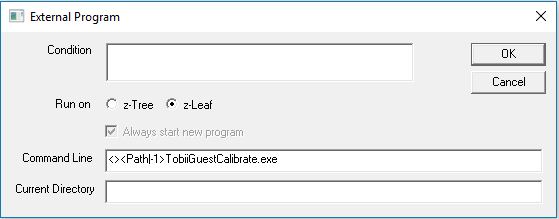
\includegraphics[width=0.6\textwidth]{ztree_extcall.png}
    \caption{External program call definition in \texttt{ztree}. The variable \texttt{Path} must be globally defined.}
    \label{fig.extcall}
\end{figure}

%------------------------------------------------------------------------------
\section{Execute 3rd Party Applications in \texttt{opensesame}}
\label{sec.external.opensesame}

Opensesame allows to run python scripts within the experiment protocols and python can be used to start external applications.
All python scripts within an opensesame experiment share the same workspace which means that a variable defined in one script will be accessible by all other scripts as well.
This can be used to define the installation path of the gaze toolset in order to avoid typing the same path multiple times.
To to this append a new item \emph{inline\_script} to the experiment and add the following lines (make sure to set the path to where the gaze toolset was installed):

\begin{lstlisting}[language=Python]
gazeToosetPath="C:\\GazeToolset"
print(f"use gaze toolset path {gazeToolsetPath}")
\end{lstlisting}

For each application to execute from within the experiment use a separate \emph{inline\_script}.
To run the \texttt{TobiiCalibration} application use the following script:

\begin{lstlisting}[language=Python]
import subprocess

print("start custom calibration")
subprocess.run([f"{gazeToolsetPath}\\TobiiCalibrate.exe]}")
print("Tobii calibration done")
\end{lstlisting}

To run the \texttt{Gaze} application use a command to run the application in the background instead of waiting for the application to terminate (note that the subject number variable is passed as an argument to the application):

\begin{lstlisting}[language=Python]
import subprocess

print("start gaze process")
subprocess.Popen([f"{gazeToolsetPath}\\Gaze.exe], "/subject", f"{var.get(u'subject_nr')}")
\end{lstlisting}

To run the GazeControl.exe of the gaze toolset use \texttt{subprocess.run} with the corresponding command argument.
For example, to gracefully terminate the \texttt{Gaze} application with \texttt{GazeControl} and the command argument \texttt{TERMINATE}, use the following script:

\begin{lstlisting}[language=Python]
import subprocess

print("stop gaze process")
subprocess.run([f"{gazeToolsetPath}\\GazeControl.exe], "/command", "TERMINATE")
\end{lstlisting}


%==============================================================================
\chapter{Configuration of the \texttt{Gaze} Toolset}
\label{sec.config}
The \texttt{Gaze} toolset can be configured to work with different installations.
It allows to specify installation paths and gives some control over implemented features (e.g.~mouse hiding or data logging).
The Listing~\ref{lst.config} shows the default configuration values and provides an explanation for each value.
The configuration file contains detailed descriptions for each parameter.
It is recommended to go through all the configuration parameters and read the description in order to get an understanding of the available configuration options.

\lstinputlisting[language=json, caption={Default configuartion values}, label=lst.config]{../sample/config.json}

Note that the configuration file follows the \texttt{json} syntax which must not be violated.
If the following points are respected, no problem should arise:
\begin{itemize}
    \item the configuration parameters are enclosed in `\texttt{\{}' and `\texttt{\}}'.
    \item all configuration parameters are of the form \texttt{"key":value} where \texttt{"key"} must not be changed.
    \item each configuration line ends with a `\texttt{,}' except for the last line where it is omitted.
    \item the Windows path delimiter `\texttt{\textbackslash}' must be escaped (i.e.~ write `\texttt{\textbackslash\textbackslash}' when describing a path)
    \item \texttt{json} supports standard data types (e.g. integer, boolean, string).
        Use the same type as the default value.
    \item everything following a `\texttt{//}' is considered a comment.
\end{itemize}

Each executable of the toolset uses the same common configuration file.
The configuration file must be named \texttt{config.json} and is read from the following places with the indicated priority:
\begin{enumerate}
    \item in the directory of the caller, i.e.~in the execution folder of the ztree client or the opensesame application
    \item in the directory of the executables, i.e.~in \texttt{<Gaze toolset path>}
\end{enumerate}
If no configuration file can be found, the application fails.

\begin{mdframed}[backgroundcolor=boxbkg]\textbf{\color{red}Warning:}
    A word of warning when using the mouse hiding feature.
    This feature hides the mouse when running \texttt{Gaze.exe}.
    If \texttt{Gaze.exe} is forcefully closed or crashes, the mouse pointer stays hidden.
    For such cases the \texttt{ShowMouse.exe} utility can be used to restore the mouse pointer.
\end{mdframed}

%------------------------------------------------------------------------------
\section{Gaze Output File}
\label{sec.output.gaze}
When running the program \texttt{Gaze.exe} an output file can be generated which holds the gaze data provided by the Tobii engine.
The output file is saved in the directory specified by \texttt{OutputPath} in \texttt{config.json}.
The name of the output file follows the form
\begin{lstlisting}
<yyyyMMddTHHmmss>_<hostName>_<ConfigName>[_<SubjectNumber>]_gaze[_err-<code>].txt
\end{lstlisting}
where
\begin{itemize}
    \item \texttt{<yyyyMMddTHHmmss>} is replaced by the timestamp indicating when the file was created (e.g. 20180129T085521 stands for 29.01.2018 08:55:21).
    \item \texttt{<hostName>} is replaced by the name of the machine
    \item \texttt{<ConfigName>} is replaced by the configuration value \texttt{"ConfigName"} as specified in the configuration file (see Listing~\ref{lst.config} for more details)
    \item \texttt{<SubjectNumber>} is replaced by the subject number passed by argument \texttt{/subject} to the application.
        If no argument \texttt{/subject} is passed the subject number is omitted in the file name (as well as the prefixed underline character).
    \item \texttt{[\_err-<code>]} is either omitted if no error occurred during the experiment or indicates data errors where
        \begin{itemize}
            \item \texttt{<code>} is replaced by an error code which is a binary string where each character can either be 1, indicating an error or 0, indicating no error (see Section~\ref{sect.data.error})
        \end{itemize}
\end{itemize}

A gaze data output file is only generated if the parameter \texttt{"DataLogWriteOutput"} in the configuration file is set to \texttt{true} (which is the default).
The presentation of the data is configurable with the help of the parameters \texttt{"DataLogColumnOrder"}, \texttt{"DataLogColumnTitle"}, \texttt{"DataLogFormatDiameter"}, \texttt{"DataLogFormatOrigin"}, and \texttt{"DataLogFormatTimeStamp"} (see Listing~\ref{lst.config} for more details).

A gaze point describes a point on the screen in x and y coordinates (pixel values) the user is gazing at.
This coordinate system is called \emph{Active Display Coordinate System (ADCS)} and is illustrated in Figure~\ref{fig.adcs}.
\begin{figure}[ht]
    \centering
    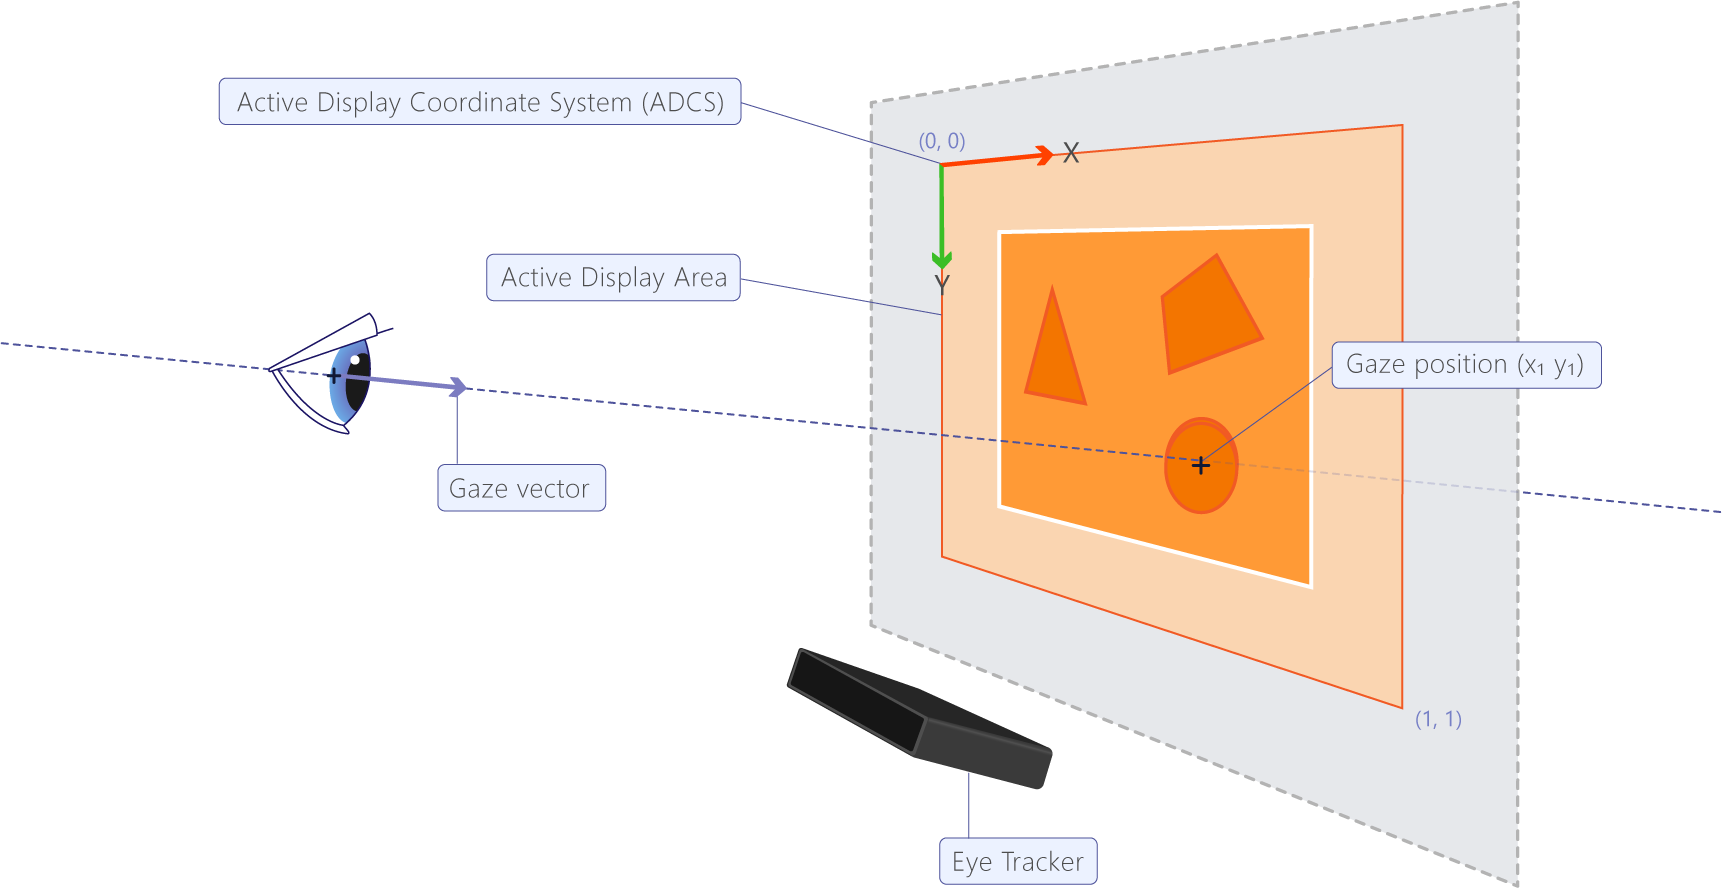
\includegraphics[width=0.8\textwidth]{adcs.png}
    \caption{The Active Display Coordinate System (ADCS). Figure source: \href{http://developer.tobiipro.com/commonconcepts/coordinatesystems.html}{Tobii}}
    \label{fig.adcs}
\end{figure}

By default, the system is configured to log all available data points.
However, this can easily be changed through the parameter \texttt{"DataLogColumnOrder"}.
For example, to only store a minimalistic set of data points use the value \texttt{"\{0\}\textbackslash t\{5\}\textbackslash t\{6\}"}.
This will only store the timestamp of when the gaze point was captured by the eye tracker (data field number 0) and the x and y coordinates of the gaze point (data field numbers 5 and 6, respectively).
This produces an output file that is similar to the following:
\lstset{columns=flexible}
\lstset{keepspaces=true}
\begin{lstlisting}
Timestamp   combined_gazePoint2d_x  combined_gazePoint2d_y
12:51:55.409    426 342
12:51:55.420    430 341
12:51:55.431    431 341
...
\end{lstlisting}

When opening the file with a spreadsheet software such as LibreOffice Calc or Microsoft Office Excel two things need to be considered:
\begin{enumerate}
    \item The column delimiter needs to be set to the delimiter set in the configuration file (\texttt{'\textbackslash t'} by default).
    \item The language needs to be set to the language of the windows system where the configuration file was produced.
        This is important because numbers are represented differently in different languages and depending on the settings, commas might be interpreted as delimiters when they are not.
\end{enumerate}

When using \href{http://developer.tobii.com/tobii-pro-sdk/}{Tobii Pro SDK}, much more values are provided and can be logged to the output file.
This includes the pupil diameters of each eye as well as the eye positions in space.
The latter uses a coordinate system which is called \emph{User Coordinate System (UCS)}.
The UCS is illustrated in Figure~\ref{fig.ucs}.
\begin{figure}[ht]
    \centering
    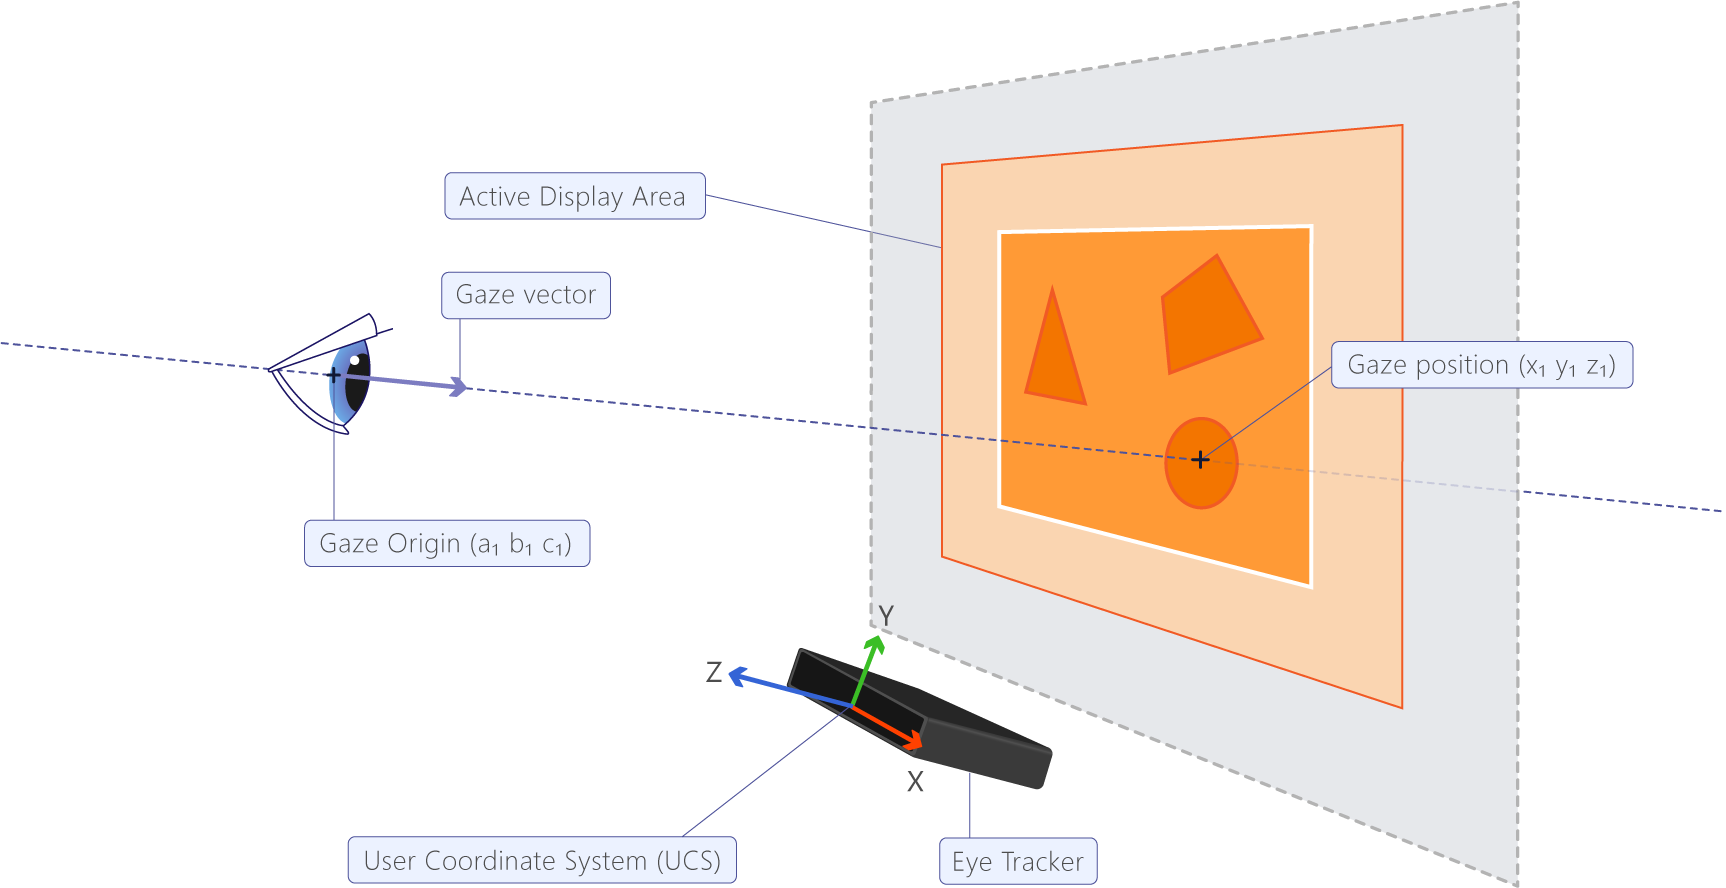
\includegraphics[width=0.8\textwidth]{ucs.png}
    \caption{The User Coordinate System (UCS). Figure source: \href{http://developer.tobiipro.com/commonconcepts/coordinatesystems.html}{Tobii}}
    \label{fig.ucs}
\end{figure}

In order to log additional data fields, the parameter \texttt{"DataLogColumnOrder"} must be modified by adding the required numbers, representing different data fields.

When using the empty string, all possible data fields are logged:
\begin{lstlisting}
"DataLogColumnOrder": ""
\end{lstlisting}

\subsection{Gaze Data Fields}
The comments above the parameter \texttt{"DataLogColumnOrder"} in the configuration file (see Listing~\ref{lst.config}) provide a short description for each available data field.
In the following some further information is provided.

The following data field types with individual data fields are provided:
\begin{enumerate}
    \item timestamps indicating when the data was sampled by the eye tracker
    \item the trial ID and an arbitrary tag to annotate each data sample
    \item 2D gaze point ADCS coordinates (see Figure~\ref{fig.adcs}) as normalized values
        \begin{description}
            \item[Mouse Tracker] \hfill
                \begin{itemize}
                    \item the x and y coordinates of the mouse pointer
                \end{itemize}
            \item[Tobii Pro SDK] \hfill
                \begin{itemize}
                    \item raw x and y coordinates of the left and the right eye
                    \item the drift compensated x and y coordinates which are computed by the drift compensation process using the I-DT algorithm for fixation detection and then comparing the averaged gaze samples to an oracle gaze to computing the drift of the gaze
                    \item the average x and y coordinates which are computed from raw data as defined by Equation~\ref{eq.average}
\begin{equation}
    \label{eq.average}
    \text{val} =
        \begin{cases}
            \text{NaN}                                      & \quad \text{if val\_right and val\_left are not valid}\\
            \text{val\_left}                                & \quad \text{if val\_right is not valid}\\
            \text{val\_right}                               & \quad \text{if val\_left is not valid}\\
            \frac{\text{val\_left} + \text{val\_right}}{2}  & \quad \text{otherwise}
        \end{cases}
\end{equation}
                \end{itemize}
        \end{description}
    \item 3D gaze point UCS coordinates (see Figure~\ref{fig.ucs}) in millimeters
        \begin{description}
            \item[Mouse Tracker] not applicable
            \item[Tobii Pro SDK] \hfill
                \begin{itemize}
                    \item raw x, y, and z coordinates of the left and the right eye
                    \item the drift compensated x, y, and z coordinates which are computed by the drift compensation process using the I-DT algorithm for fixation detection and then comparing the averaged gaze samples to an oracle gaze to computing the drift of the gaze
                    \item the average x and y coordinates which are computed from raw data as defined by Equation~\ref{eq.average}
                \end{itemize}
        \end{description}
    \item gaze origin UCS coordinates (see Figure~\ref{fig.ucs}) in millimetres
        \begin{description}
            \item[Mouse Tracker] not applicable
            \item[Tobii Pro SDK] \hfill
                \begin{itemize}
                    \item raw x, y, and z coordinates of the left and the right eye
                    \item the average x, y, and z coordinates which are computed from raw data as defined by Equation~\ref{eq.average}
                    \item the distance from the gaze origin to the left and the right gaze point, respectively which are computed from raw data as defined by Equation~\ref{eq.dist}
\begin{equation}
    \label{eq.dist}
    \text{dist} = \sqrt{x^2 + y^2 + z^2}
\end{equation}
                    \item the average distance which is computed from the distance of the left and the right eye as defined by Equation~\ref{eq.average}
                \end{itemize}
        \end{description}
    \item pupil diameters in millimetres
        \begin{description}
            \item[Mouse Tracker] not applicable
            \item[Tobii Pro SDK] \hfill
                \begin{itemize}
                    \item raw diameters of the left and the right eye
                    \item the average diameter which is computed from raw data as defined by Equation~\ref{eq.average}
                \end{itemize}
        \end{description}
    \item data validity indicators as true or false
        \begin{description}
            \item[Mouse Tracker] not supported
            \item[Tobii Pro SDK] \hfill
                \begin{itemize}
                    \item separate values that indicate whether gaze points, gaze origins, and pupil diameters are valid for combined values, the left and the right eye, respectively
                \end{itemize}
        \end{description}
\end{enumerate}

\begin{mdframed}[backgroundcolor=boxbkg]\textbf{\color{orange}Notice:}
    The time resolution of the mouse tracker device is rather poor (15 milliseconds).
    Therefore it can happen that multiple mouse events are logged with the same timestamp.
\end{mdframed}

\subsection{Gaze Data Timestamps and Annotations}
\label{sect.data.annotations}
Gaze data have three different timestamps:
\begin{description}
    \item[timestamp] The system time when the data point was captured by the device.
    \item[timestamp\_received] The system time when the data point was received by the system.
    \item[Timestamp\_relative] The number of milliseconds since the start of the application.
        Note that this timestamp can be reset with the command \texttt{GazeControl.exe /reset}.
\end{description}

The latency of the gaze data can computed with Equation~\ref{eq.latency}.
\begin{equation}
    \label{eq.latency}
    latency = timestamp\_received - timestamp
\end{equation}

Gaze data can be annotated with a \texttt{label} and a \texttt{trial ID}.
To do this use the command \texttt{GazeControl.exe /label <label>} and \texttt{GazeControl.exe /trialID <ID of the trial>}, respectively.
A label can be any arbitrary string (make sure to use quotations marks in the command if the label has spaces).
The trial ID must be an integer number.
The label and trial ID annotations are assigned to gaze data points synchronized with the timestamp when the data was captured.
This means that when a label or a trial ID is set through a command, the gaze data is not annotated immediately.
Rather, the annotations are delayed such that the timestamps are synchronized with the timestamps of the data capture.

\subsection{Gaze Data Error Code}
\label{sect.data.error}
The data error code that is postfixed to the output file name is a binary string where each character indicates whether a specific error has occurred (indicated with the number \texttt{1}) or not (indicated with the number \texttt{0}).
Multiple errors can occur at the same time, hence, the position of a \texttt{1} in the error code indicates the specific error.
If all positions of the error code are 0, the errors are not postfixed to the output file name.

The following list describes the individual errors that can occur during an experiment:
\begin{description}
    \item[code \texttt{10}] \hfill \\
        This code indicates that during the experiment the eye tracker device stopped tracking.
        This means that in the output file gaze data is potentially missing.
        This can be caused by a malfunctioning of the eye tracker device or simply because the device was disconnected.
        The exact time instances of such an occurrence is logged to the log file.
    \item[code \texttt{01}] \hfill \\
        This code indicates that the system had to fall back to the Mouse Tracker.
        This error occurs if the system was configured to use the \href{http://developer.tobii.com/tobii-pro-sdk/}{Tobii Pro SDK} but was not able to do so.
        This usually happens when the license file is not accessible.
        Check whether the license files are accessible by the system and whether the license path is correctly defined in parameter \texttt{"LicensePath"}.
\end{description}

%------------------------------------------------------------------------------
\section{Calibration Output File}
When running the program \texttt{GazeControl.exe /command CUSTOM\_CALIBRATE} an output file can be generated which holds the calibration results provided by the Tobii engine.
The output file is saved in the directory specified by \texttt{OutputPath} in \texttt{config.json}.
The name of the output file follows the form
\begin{lstlisting}
<yyyyMMddTHHmmss>_<hostName>_<ConfigName>[_<SubjectNumber>]_calibration[_err-<code>].txt
\end{lstlisting}
where
\begin{itemize}
    \item \texttt{<yyyyMMddTHHmmss>} is replaced by the timestamp indicating when the file was created (e.g. 20180129T085521 stands for 29.01.2018 08:55:21).
    \item \texttt{<hostName>} is replaced by the name of the machine
    \item \texttt{<ConfigName>} is replaced by the configuration value \texttt{"ConfigName"} as specified in the configuration file (see Listing~\ref{lst.config} for more details)
    \item \texttt{<SubjectNumber>} is replaced by the subject number passed by argument \texttt{/subject} to the application.
        If no argument \texttt{/subject} is passed the subject number is omitted in the file name (as well as the prefixed underline character).
    \item \texttt{[\_err-<code>]} is either omitted if no error occurred during the experiment or indicates data errors where
        \begin{itemize}
            \item \texttt{<code>} is replaced by an error code which is a binary string where each character can either be 1, indicating an error or 0, indicating no error (see Section~\ref{sect.calibration.error})
        \end{itemize}
\end{itemize}

A calibration output file is only generated if the parameter \texttt{"CalibrationLogWriteOutput"} in the configuration file is set to \texttt{true} (which is the default).

The configuration of the calibration data fields to be stored to the output file follows the same logic as described with the gaze output in Section \ref{sec.output.gaze}, except that the presentation of the data is defined through parameters \texttt{"CalibrationLogColumnOrder"}, \texttt{"CalibrationColumnTitle"}, \texttt{"DataLogFormatNormalizedPoint"}, and \texttt{"DataLogFormatTimeStamp"} (see Listing~\ref{lst.config} for more details).

\subsection{Calibration Data Fields}
The comments above the parameter \texttt{"CalibrationLogColumnOrder"} in the configuration file (see Listing~\ref{lst.config}) provide a short description for each available data field.
In the following some further information is provided.

The following three data field types with individual data fields are provided:
\begin{enumerate}
    \item calibration point ADCS coordinates (see Figure~\ref{fig.adcs}) as normalized values
        \begin{description}
            \item[Mouse Tracker] not applicable
            \item[Tobii Pro SDK] \hfill
                \begin{itemize}
                    \item x and y coordinates of the calibration point
                \end{itemize}
        \end{description}
    \item gaze point ADCS coordinates (see Figure~\ref{fig.adcs}) as normalized values
        \begin{description}
            \item[Mouse Tracker] not applicable
            \item[Tobii Pro SDK] \hfill
                \begin{itemize}
                    \item x and y coordinates of the gaze point of the left and right eye
                \end{itemize}
        \end{description}
    \item data validity indicators as either \texttt{ValidAndUsed}, \texttt{ValidAndUnused}, and \texttt{Invalid}
        \begin{description}
            \item[Mouse Tracker] not supported
            \item[Tobii Pro SDK] \hfill
                \begin{itemize}
                    \item separate values that indicate whether gaze points are valid for the left and the right eye, respectively
                \end{itemize}
        \end{description}
\end{enumerate}

\subsection{Calibration Data Error Code}
\label{sect.calibration.error}
The error code that is postfixed to the calibration output file name is a binary string where each character indicates whether a specific error has occurred (indicated with the number \texttt{1}) or not (indicated with the number \texttt{0}).
Multiple errors can occur at the same time, hence, the position of a \texttt{1} in the error code indicates the specific error.
If all positions of the error code are 0, the errors are not postfixed to the output file name.

The following list describes the individual errors that can occur during an experiment:
\begin{description}
    \item[code \texttt{10}] \hfill \\
        This code indicates that during the calibration the eye tracker device stopped tracking.
        This means that the calibration had to be redone in order to be valid.
        This can be caused by a malfunctioning of the eye tracker device or simply because the device was disconnected.
        The exact time instances of such an occurrence is logged to the log file.
    \item[code \texttt{01}] \hfill \\
        This code indicates that the system was not able to start the calibration because the device does not support calibration.
        This error occurs if the configuration option \texttt{TrackerDevice} was set to a device with no calibration support.
\end{description}


%------------------------------------------------------------------------------
\section{Validation Output File}
When running the program \texttt{GazeControl.exe /command VALIDATE} an output file can be generated which holds the validation results provided by the Tobii engine.
The output file is saved in the directory specified by \texttt{OutputPath} in \texttt{config.json}.
The name of the output file follows the form
\begin{lstlisting}
<yyyyMMddTHHmmss>_<hostName>_<ConfigName>[_<SubjectNumber>]_validation[_err-<code>].txt
\end{lstlisting}
where
\begin{itemize}
    \item \texttt{<yyyyMMddTHHmmss>} is replaced by the timestamp indicating when the file was created (e.g. 20180129T085521 stands for 29.01.2018 08:55:21).
    \item \texttt{<hostName>} is replaced by the name of the machine
    \item \texttt{<ConfigName>} is replaced by the configuration value \texttt{"ConfigName"} as specified in the configuration file (see Listing~\ref{lst.config} for more details)
    \item \texttt{<SubjectNumber>} is replaced by the subject number passed by argument \texttt{/subject} to the application.
        If no argument \texttt{/subject} is passed the subject number is omitted in the file name (as well as the prefixed underline character).
    \item \texttt{[\_err-<code>]} is either omitted if no error occurred during the experiment or indicates data errors where
        \begin{itemize}
            \item \texttt{<code>} is replaced by an error code which is a binary string where each character can either be 1, indicating an error or 0, indicating no error (see Section~\ref{sect.calibration.error})
        \end{itemize}
\end{itemize}

A validation output file is only generated if the parameter \texttt{ValidationLogWriteOutput"} in the configuration file is set to \texttt{true} (which is the default).

The configuration of the validation data fields to be stored to the output file follows the same logic as described with the gaze output in Section \ref{sec.output.gaze}, except that the presentation of the data is defined through parameters \texttt{"ValidationLogColumnOrder"} and \texttt{"ValidationColumnTitle"} (see Listing~\ref{lst.config} for more details).

\subsection{Validation Data Fields}
The comments above the parameter \texttt{"ValidationLogColumnOrder"} in the configuration file (see Listing~\ref{lst.config}) provide a short description for each available data field.
In the following some further information is provided.

The following three data fields are provided for the left and the right eye:
\begin{enumerate}
    \item validation point ADCS coordinates (see Figure~\ref{fig.adcs}) as normalized values
        \begin{description}
            \item[Mouse Tracker] not applicable
            \item[Tobii Pro SDK] \hfill
                \begin{itemize}
                    \item x and y coordinates of the validation point
                \end{itemize}
        \end{description}
    \item accuracy of the gaze points.
        \begin{description}
            \item[Mouse Tracker] not applicable
            \item[Tobii Pro SDK] \hfill
                \begin{itemize}
                    \item systematic error of the measured gaze point with respect to the target gaze point in degrees
                \end{itemize}
        \end{description}
    \item precision of the gaze points
        \begin{description}
            \item[Mouse Tracker] not applicable
            \item[Tobii Pro SDK] \hfill
                \begin{itemize}
                    \item averaged standard deviation over all collected points in degrees
                \end{itemize}
        \end{description}
    \item precision RMS
        \begin{description}
            \item[Mouse Tracker] not supported
            \item[Tobii Pro SDK] \hfill
                \begin{itemize}
                    \item averaged root mean square of sample-to-sample error over all collected points in degrees
                \end{itemize}
        \end{description}
\end{enumerate}

\subsection{Validation Data Error Code}
\label{sect.validation.error}
The error code that is postfixed to the validation output file name is a binary string where each character indicates whether a specific error has occurred (indicated with the number \texttt{1}) or not (indicated with the number \texttt{0}).
Multiple errors can occur at the same time, hence, the position of a \texttt{1} in the error code indicates the specific error.
If all positions of the error code are 0, the errors are not postfixed to the output file name.

The following list describes the individual errors that can occur during an experiment:
\begin{description}
    \item[code \texttt{10}] \hfill \\
        This code indicates that during the validation the eye tracker device stopped tracking.
        This means that the validation had to be redone in order to be valid.
        This can be caused by a malfunctioning of the eye tracker device or simply because the device was disconnected.
        The exact time instances of such an occurrence is logged to the log file.
    \item[code \texttt{01}] \hfill \\
        This code indicates that the system was not able to start the validation because the device does not support validation.
        This error occurs if the configuration option \texttt{TrackerDevice} was set to a device with no validation support.
\end{description}

%------------------------------------------------------------------------------
\section{Configuration File Dump}
For each experiment where the utility \texttt{Gaze.exe} is executed, a dump of the configuration file is produced.
This allows to associate a set of configuration values to an experiment, reuse the same configuration file should the experiment be repeated, and provides transparency of how the output data was produced.
Note that in this configuration file all comments are omitted and the formatting (indentations, white spaces, carriage return) is removed.
To reformat the file or display the file as a tree structure, online tools, such as the \href{http://jsonviewer.stack.hu/}{Online JSON Viewer}\footnote{http://jsonviewer.stack.hu/}, can be used.

The name of the dumped configuration file is of the form
\begin{lstlisting}
<yyyyMMddTHHmmss>_<hostName>_<ConfigName>_config[_err-<code>-<code>].txt
\end{lstlisting}
where
\begin{itemize}
    \item \texttt{<yyyyMMddTHHmmss>} is replaced by the timestamp indicating when the file was created (e.g. 20180129T085521 stands for 29.01.2018 08:55:21)
    \item \texttt{<hostName>} is replaced by the name of the machine
    \item \texttt{<ConfigName>} is replaced by the configuration value \texttt{"ConfigName"} as specified in the configuration file (see Listing~\ref{lst.config} for more details)
    \item \texttt{[\_err-<code>-<code>]} is either omitted if no error occurred during the experiment or indicates data errors where
        \begin{itemize}
            \item \texttt{<code>} is replaced by an error code which is a binary string where each character can either be 1, indicating an error or 0, indicating no error (see Section~\ref{sect.config.error})
        \end{itemize}
\end{itemize}

In addition to the configuration data used during the experimentation the dumped configuration file includes information on the screen area in UCS coordinate system (see Figure~\ref{fig.ucs}).
The Listing~\ref{lst.screen} shows an example of the screen area data as it can be found in the dumped configuration file.

\begin{lstlisting}[language=json, caption={Screen Area Data in Dumped Config}, label=lst.screen]
{
  "ScreenArea": {
    "Width": 597.5177001953125,
    "Height": 336.10369873046875,
    "Center": [
      0.1185302734375,
      173.82257080078125,
      56.42921829223633
    ],
    "TopLeft": [
      -298.64031982421875,
      331.7396545410156,
      113.90633392333984
    ],
    "TopRight": [
      298.87738037109375,
      331.7396545410156,
      113.90633392333984
    ],
    "BottomLeft": [
      -298.64031982421875,
      15.905486106872559,
      -1.0478993654251099
    ],
    "BottomRight": [
      298.87738037109375,
      15.905486106872559,
      -1.0478993654251099
    ]
  }
}
\end{lstlisting}

\subsection{Configuration Error Code}
\label{sect.config.error}
The configuration error codes that are postfixed to the dumped configuration file name are binary strings where each character indicates whether a specific error has occurred (indicated with the number \texttt{1}) or not (indicated with the number \texttt{0}).
Multiple errors can occur at the same time, hence, the position of a \texttt{1} in the error code indicates the specific error.
If all positions of all error codes are 0, the errors are not postfixed to the dumped configuration file.

The following list describes the individual errors of the first error code that addresses general problems with the configuration file:
\begin{description}
    \item[code \texttt{100}] \hfill \\
        The system ignores the configuration file and falls back to the default configuration values.
        This happens if an invalid configuration file is provided that cannot be parsed.
        Verify the syntax of the configuration file and make sure that the key names are not modified and no additional keys are added to the file.
        Note that it is perfectly valid to not provide a configuration file which causes the system to use the default values without creating an error.
    \item[code \texttt{010}] \hfill \\
        The system uses the current location (e.g. \texttt{<zleaf path>}) to store the output files.
        This happens if the provided path in the configuration file (parameter \texttt{"DataLogPath"}) is invalid or non-existent.
        Verify that the provided path exists and that no invalid characters are used (do not use \texttt{<>:"/\textbackslash |?}).
    \item[code \texttt{001}] \hfill \\
        This happens if no name was provided or the provided name in the configuration file (parameter \texttt{"ConfigName"}) is invalid.
        The configuration name is mandatory and the application failed due to this error.
        Verify that in the provided name no invalid characters are used (do not use \texttt{<>:"/\textbackslash |?}).
\end{description}

The following list describes the individual errors of the second error code that specifically addresses problems concerning the formatting of the output file:
\begin{description}
    \item[code \texttt{010000}] \hfill \\
        The system falls back to the default column order.
        This happens if the parameter \texttt{"DataLogColumnOrder"} is invalid.
        Make sure that only existing data filed numbers are used and that the format string is valid.
        More information on format strings is provided on the MSDN page about \href{https://docs.microsoft.com/en-us/dotnet/standard/base-types/composite-formatting}{Composite Formatting}\footnote{https://docs.microsoft.com/en-us/dotnet/standard/base-types/composite-formatting}.
    \item[code \texttt{001000}] \hfill \\
        The column titles are not printed to the output file.
        This happens if the value of parameter \texttt{"DataLogColumnTitle"} is not valid.
        Make sure that a title is provided for all possible data fields (not only the ones that are displayed).
    \item[code \texttt{000100}] \hfill \\
        The system falls back to the default format for the timestamp.
        This happens if the value provided for the parameter \texttt{"DataLogFormatTimeStamp"} is invalid.
        Refer to the MSDN page about \href{https://docs.microsoft.com/en-us/dotnet/standard/base-types/formatting-types}{Formatting Types}\footnote{https://docs.microsoft.com/en-us/dotnet/standard/base-types/formatting-types} for more information.
    \item[code \texttt{000010}] \hfill \\
        The system falls back to the default format for the gaze origin coordinates.
        This happens if the value provided for the parameter \texttt{"DataLogFormatOrigin"} is invalid.
        Refer to the MSDN page about \href{https://docs.microsoft.com/en-us/dotnet/standard/base-types/formatting-types}{Formatting Types}\footnotemark[\value{footnote}] for more information.
    \item[code \texttt{000001}] \hfill \\
        The system falls back to the default format for the diameter of the pupil.
        This happens if the value provided for the parameter \texttt{"DataLogFormatDiameter"} is invalid.
        Refer to the MSDN page about \href{https://docs.microsoft.com/en-us/dotnet/standard/base-types/formatting-types}{Formatting Types}\footnote{https://docs.microsoft.com/en-us/dotnet/standard/base-types/formatting-types} for more information.
    \item[code \texttt{100000}] \hfill \\
        The system falls back to the default format for the normalized coordination point.
        This happens if the value provided for the parameter \texttt{"DataLogNormalizedPoint"} is invalid.
        Refer to the MSDN page about \href{https://docs.microsoft.com/en-us/dotnet/standard/base-types/formatting-types}{Formatting Types}\footnote{https://docs.microsoft.com/en-us/dotnet/standard/base-types/formatting-types} for more information.
\end{description}

%------------------------------------------------------------------------------
\section{Log File}
All executables write continuously to the same log file.
This allows to track the eye tracker events that happened throughout a session within one log file.
The log file is produced at the root directory of the application which is making the calls to the executables (e.g. at the location of zleaf.exe: \texttt{<zleaf path>}).
The name of the log file is of the form \texttt{<hostName>\_gaze.log} where \texttt{<hostName>} is replaced by the name of the machine.

\end{document}
